% https://www.mdpi.com/journal/applsci/special_issues/Machine_Learning_Acoustical_Problems#info


%  LaTeX support: latex@mdpi.com 
%  In case you need support, please attach all files that are necessary for compiling as well as the log file, and specify the details of your LaTeX setup (which operating system and LaTeX version / tools you are using).

%=================================================================
\documentclass[applsci,article,submit,oneauthor,pdftex]{Definitions/mdpi} 

% If you would like to post an early version of this manuscript as a preprint, you may use preprint as the journal and change 'submit' to 'accept'. The document class line would be, e.g.,
%\documentclass[preprints,article,accept,moreauthors,pdftex]{Definitions/mdpi}
%. This is especially recommended for submission to arXiv, where line numbers should be removed before posting. For preprints.org, the editorial staff will make this change immediately prior to posting.

%--------------------
% Class Options:
%--------------------
%----------
% journal
%----------
% Choose between the following MDPI journals:
% acoustics, actuators, addictions, admsci, aerospace, agriculture, agriengineering, agronomy, algorithms, animals, antibiotics, antibodies, antioxidants, applsci, arts, asc, asi, atmosphere, atoms, axioms, batteries, bdcc, behavsci , beverages, bioengineering, biology, biomedicines, biomimetics, biomolecules, biosensors, brainsci , buildings, cancers, carbon , catalysts, cells, ceramics, challenges, chemengineering, chemistry, chemosensors, children, cleantechnol, climate, clockssleep, cmd, coatings, colloids, computation, computers, condensedmatter, cosmetics, cryptography, crystals, dairy, data, dentistry, designs , diagnostics, diseases, diversity, drones, econometrics, economies, education, ejihpe, electrochem, electronics, energies, entropy, environments, epigenomes, est, fermentation, fibers, fire, fishes, fluids, foods, forecasting, forests, fractalfract, futureinternet, futurephys, galaxies, games, gastrointestdisord, gels, genealogy, genes, geohazards, geosciences, geriatrics, hazardousmatters, healthcare, heritage, highthroughput, horticulturae, humanities, hydrology, ijerph, ijfs, ijgi, ijms, ijns, ijtpp, informatics, information, infrastructures, inorganics, insects, instruments, inventions, iot, j, jcdd, jcm, jcp, jcs, jdb, jfb, jfmk, jimaging, jintelligence, jlpea, jmmp, jmse, jnt, jof, joitmc, jpm, jrfm, jsan, land, languages, laws, life, literature, logistics, lubricants, machines, magnetochemistry, make, marinedrugs, materials, mathematics, mca, medicina, medicines, medsci, membranes, metabolites, metals, microarrays, micromachines, microorganisms, minerals, modelling, molbank, molecules, mps, mti, nanomaterials, ncrna, neuroglia, nitrogen, notspecified, nutrients, ohbm, optics, particles, pathogens, pharmaceuticals, pharmaceutics, pharmacy, philosophies, photonics, physics, plants, plasma, polymers, polysaccharides, preprints , proceedings, processes, proteomes, psych, publications, quantumrep, quaternary, qubs, reactions, recycling, religions, remotesensing, reports, resources, risks, robotics, safety, sci, scipharm, sensors, separations, sexes, signals, sinusitis, smartcities, sna, societies, socsci, soilsystems, sports, standards, stats, surfaces, surgeries, sustainability, symmetry, systems, technologies, test, toxics, toxins, tropicalmed, universe, urbansci, vaccines, vehicles, vetsci, vibration, viruses, vision, water, wem, wevj

%---------
% article
%---------
% The default type of manuscript is "article", but can be replaced by: 
% abstract, addendum, article, benchmark, book, bookreview, briefreport, casereport, changes, comment, commentary, communication, conceptpaper, conferenceproceedings, correction, conferencereport, expressionofconcern, extendedabstract, meetingreport, creative, datadescriptor, discussion, editorial, essay, erratum, hypothesis, interestingimages, letter, meetingreport, newbookreceived, obituary, opinion, projectreport, reply, retraction, review, perspective, protocol, shortnote, supfile, technicalnote, viewpoint
% supfile = supplementary materials

%----------
% submit
%----------
% The class option "submit" will be changed to "accept" by the Editorial Office when the paper is accepted. This will only make changes to the frontpage (e.g., the logo of the journal will get visible), the headings, and the copyright information. Also, line numbering will be removed. Journal info and pagination for accepted papers will also be assigned by the Editorial Office.

%------------------
% moreauthors
%------------------
% If there is only one author the class option oneauthor should be used. Otherwise use the class option moreauthors.

%---------
% pdftex
%---------
% The option pdftex is for use with pdfLaTeX. If eps figures are used, remove the option pdftex and use LaTeX and dvi2pdf.

%=================================================================
\firstpage{1} 
\makeatletter 
\setcounter{page}{\@firstpage} 
\makeatother
\pubvolume{xx}
\issuenum{1}
\articlenumber{5}
\pubyear{2019}
\copyrightyear{2019}
%\externaleditor{Academic Editor: name}
\history{Received: date; Accepted: date; Published: date}
%\updates{yes} % If there is an update available, un-comment this line

%% MDPI internal command: uncomment if new journal that already uses continuous page numbers 
%\continuouspages{yes}

%------------------------------------------------------------------
% The following line should be uncommented if the LaTeX file is uploaded to arXiv.org
%\pdfoutput=1

%=================================================================
% Add packages and commands here. The following packages are loaded in our class file: fontenc, calc, indentfirst, fancyhdr, graphicx, lastpage, ifthen, lineno, float, amsmath, setspace, enumitem, mathpazo, booktabs, titlesec, etoolbox, amsthm, hyphenat, natbib, hyperref, footmisc, geometry, caption, url, mdframed, tabto, soul, multirow, microtype, tikz

%=================================================================
%% Please use the following mathematics environments: Theorem, Lemma, Corollary, Proposition, Characterization, Property, Problem, Example, ExamplesandDefinitions, Hypothesis, Remark, Definition, Notation, Assumption
%% For proofs, please use the proof environment (the amsthm package is loaded by the MDPI class).

%================\usepackage[cmex10]{amsmath}
%Mathabx do not work on ScribTex => Removed
%\usepackage{mathabx}
\usepackage{array}
\usepackage{mdwmath}
\usepackage{mdwtab}
\usepackage{eqparbox}
\usepackage{url}
\usepackage{cite}
\usepackage{amsmath,amssymb,amsfonts}
\usepackage{algorithmic}
\usepackage{graphicx}
\usepackage{textcomp}
\usepackage{xcolor}

\newcommand{\etal}{{et al}.\@ }
\newcommand{\iec}{i.\,e.,\ }
\newcommand{\ie}{i.\,e.\ }
\newcommand{\egc}{e.\,g.,\ }
\newcommand{\eg}{e.\,g.\ }
% \newcommand{\chapref}[1]{{Chapter \ref{#1}}}
% \newcommand{\partref}[1]{{Part \ref{#1}}}
\newcommand{\figref}[1]{{Figure \ref{#1}}}
\newcommand{\secref}[1]{{Section \ref{#1}}}
\newcommand{\tabref}[1]{{Table \ref{#1}}}
\newcommand{\eqnref}[1]{{Equation \ref{#1}}}


% Full title of the paper (Capitalized)
\Title{A Review of Approaches and Challenges for Acoustic Scene Classification}

% Author Orchid ID: enter ID or remove command
\newcommand{\orcidauthorA}{0000-0003-4689-7944} % Add \orcidA{} behind the author's name
%\newcommand{\orcidauthorB}{0000-0000-000-000X} % Add \orcidB{} behind the author's name

% Authors, for the paper (add full first names)
\Author{Jakob Abe{\ss}er $^1$\orcidA{}
%, Stylianos I. Mimilakis $^{2}$
}

% Authors, for metadata in PDF
\AuthorNames{Jakob Abe{\ss}er
%, Stylianos I. Mimilakis
}

% Affiliations / Addresses (Add [1] after \address if there is only one affiliation.)
\address{%
$^{1}$ \quad Semantic Music Technologies, Fraunhofer IDMT, Ehrenbergstra{\ss}e 31, 98693 Ilmenau, Germany; jakob.abesser@idmt.fraunhofer.de%\\
%$^{2}$ \quad Fraunhofer IDMT; stylianos.ioannis.mimilakis@idmt.fraunhofer.de
}

% Contact information of the corresponding author
\corres{Correspondence: jakob.abesser@idmt.fraunhofer.de}

% Current address and/or shared authorship
%\firstnote{Current address: Affiliation 3} 
%\secondnote{These authors contributed equally to this work.}
% The commands \thirdnote{} till \eighthnote{} are available for further notes

%\simplesumm{} % Simple summary

%\conference{} % An extended version of a conference paper
\abstract{The number of publications on acoustic scene classification (ASC) in environmental audio recordings constantly increased over the last years.
This was mainly stimulated by the annual Detection and Classification of Acoustic Scenes and Events (DCASE) competition with its first edition in 2013.
All competitions so far involved one or multiple ASC tasks. % and various datasets were used over the years.
With a focus on deep learning-based ASC algorithms, this article summarizes and groups existing approaches for data preparation, \iec feature representations, feature pre-processing, and data augmentation, and for data modelling, \iec neural network architectures and learning paradigms.
Finally, the paper discusses current algorithmic limitations and open challenges in order to preview possible future developments towards the real-life application of ASC systems.}

% Keywords
\keyword{acoustic scene classification, machine listening, deep neural networks} % TODO add third one

% The fields PACS, MSC, and JEL may be left empty or commented out if not applicable
%\PACS{J0101}
%\MSC{}
%\JEL{}

%%%%%%%%%%%%%%%%%%%%%%%%%%%%%%%%%%%%%%%%%%
% Only for the journal Diversity
%\LSID{\url{http://}}

%%%%%%%%%%%%%%%%%%%%%%%%%%%%%%%%%%%%%%%%%%
% Only for the journal Applied Sciences:
%\featuredapplication{Authors are encouraged to provide a concise description of the specific application or a potential application of the work. This section is not mandatory.}
%%%%%%%%%%%%%%%%%%%%%%%%%%%%%%%%%%%%%%%%%%

%%%%%%%%%%%%%%%%%%%%%%%%%%%%%%%%%%%%%%%%%%
% Only for the journal Data:
%\dataset{DOI number or link to the deposited data set in cases where the data set is published or set to be published separately. If the data set is submitted and will be published as a supplement to this paper in the journal Data, this field will be filled by the editors of the journal. In this case, please make sure to submit the data set as a supplement when entering your manuscript into our manuscript editorial system.}

%\datasetlicense{license under which the data set is made available (CC0, CC-BY, CC-BY-SA, CC-BY-NC, etc.)}

%%%%%%%%%%%%%%%%%%%%%%%%%%%%%%%%%%%%%%%%%%
% Only for the journal Toxins
%\keycontribution{The breakthroughs or highlights of the manuscript. Authors can write one or two sentences to describe the most important part of the paper.}

%\setcounter{secnumdepth}{4}
%%%%%%%%%%%%%%%%%%%%%%%%%%%%%%%%%%%%%%%%%%
\begin{document}
%%%%%%%%%%%%%%%%%%%%%%%%%%%%%%%%%%%%%%%%%%

% -------------------------------------
% -------------------------------------
\section{Introduction}
% -------------------------------------
% -------------------------------------

%The task of acoustic scene classification (ASC) involves to recognize, summarize, and label \textit{multiple simultaneously occurring sound events} as \textit{acoustic scenes} \citep{Virtanen:2018:SoundSceneBook:BOOK}. Acoustic scene classes cover outdoor scenes such as nature environments or public places, indoor scenes like offices or apartments, and specific vehicle types such as cars, trams, or trains. Sound events of interest range from nature sounds like bird calls, rustling leaves, and rain drops, over machine-made sounds like motor engines, braking noises, or chainsaws, to human sounds like voice, laughter, or screams. These sounds are often unstructured, non-stationary, and lack a predictable and repetitive nature. At the same time, they are composed of diverse acoustic building blocks such as short transients, noise, as well as harmonic signal components. Depending on their position within the \textit{recording location}, sound events appear either in the foreground or background.
Recognizing different indoor and outdoor acoustic environments 
%such as outdoor scenes, offices, or apartments 
from recorded acoustic signals is an active research field that has received a lot of attention in the last years. The task is an essential part of auditory scene analysis and 
%of recognition  RECOGNITION IS REPEATED
involves summarizing an entire recorded acoustic signal using a pre-defined semantic description
%~\citep{Virtanen:2018:SoundSceneBook:BOOK}, 
like ``office room'' or ``public place''. 
%In relevant research, t
Those semantic entities are denoted as \textit{acoustic scenes}, and the task of recognizing them as acoustic scene classification (ASC) \citep{Virtanen:2018:SoundSceneBook:BOOK}.

%ASC is mutually dependent with the \textit{acoustic event detection} (AED) task, which deals with the classification and temporal detection of audible sound events within an audio recording. Expert knowledge about the detected acoustic scene allows to focus on the sound events typical for this class. At the same time, knowledge about predominant sound events can facilitate the ASC task.
% While ASD provides a summarative classification of an acoustic scene, AED focuses on the precise detection of particular sound events.
A particularly challenging task related to ASC is the detection 
%and pin pointing 
of audio events which are temporarily present in an acoustic scene.
%of a test recording.
Examples of such audio events include vehicles, car horns, and footsteps among others. This task is referred to as \textit{acoustic event detection} (AED) and it substantially differs from ASC 
as it focuses
%by focusing 
on the precise temporal detection of particular sound events.
%from within an acoustic scene.

%State-of-the-art ASC algorithms have many \textit{application scenarios} in context-aware devices as they have been shown to outperform humans in recognizing acoustic scenes \citep{Mesaros:2017:HumanASC:WASPAA}. Such scenarios range from hearing aids, IoT and smart cities applications, automous navigation, wild-life monitoring in nature conservation areas to monitoring devices for physically challenged persons or persons in need of care.
% TODO add references as examples 
%Maybe cite Estefania's Annia's paper here?
State-of-the-art ASC systems have been shown to outperform humans on this task~\citep{Mesaros:2017:HumanASC:WASPAA}.
Therefore, they are applied in numerous \textit{application scenarios} such as context-aware  wearables and hearables, hearing aids, 
health care, security surveillance, wild-life monitoring in nature habitats, smart cities, IoT, and autonomous navigation. 

As current ASC methods are consistently based on deep neural networks \citep{Virtanen:2018:SoundSceneBook:BOOK}, this article summarizes the recent methodological advances in the field of deep learning based ASC. Existing methods are summarized and categorized based on the typical processing steps illustrated in 
\figref{fig:flowchart}. \secref{sec:feature_representations},  \secref{sec:feature_pre_processing}, and \secref{sec:data_augmentation} discuss techniques to represent, pre-process, and augment audio signals for ASC.
Commonly used neural network architectures and learning paradigms are detailed in \secref{sec:network_architectures} and \secref{sec:learning_paradigms}.
Finally, \secref{sec:open_challenges} discusses open challenges and limitations of current ASC algorithms before \secref{sec:conclusion} concludes this article.
Methodologies and common datasets for evaluating ASC algorithms are not further addressed in this article. The interesting reader is referred to \citep{Virtanen:2018:SoundSceneBook:BOOK, Mesaros:2016:ASC:IEEE_TASLP} and the DCASE community website\footnote{\url{http://dcase.community/}}.

% TODO
%% add refs to 
%https://arxiv.org/pdf/1905.00078.pdf

% https://research-repository.uwa.edu.au/en/publications/a-survey-neural-network-based-deep-learning-for-acoustic-event-de


\begin{figure}[t]
    \centering
    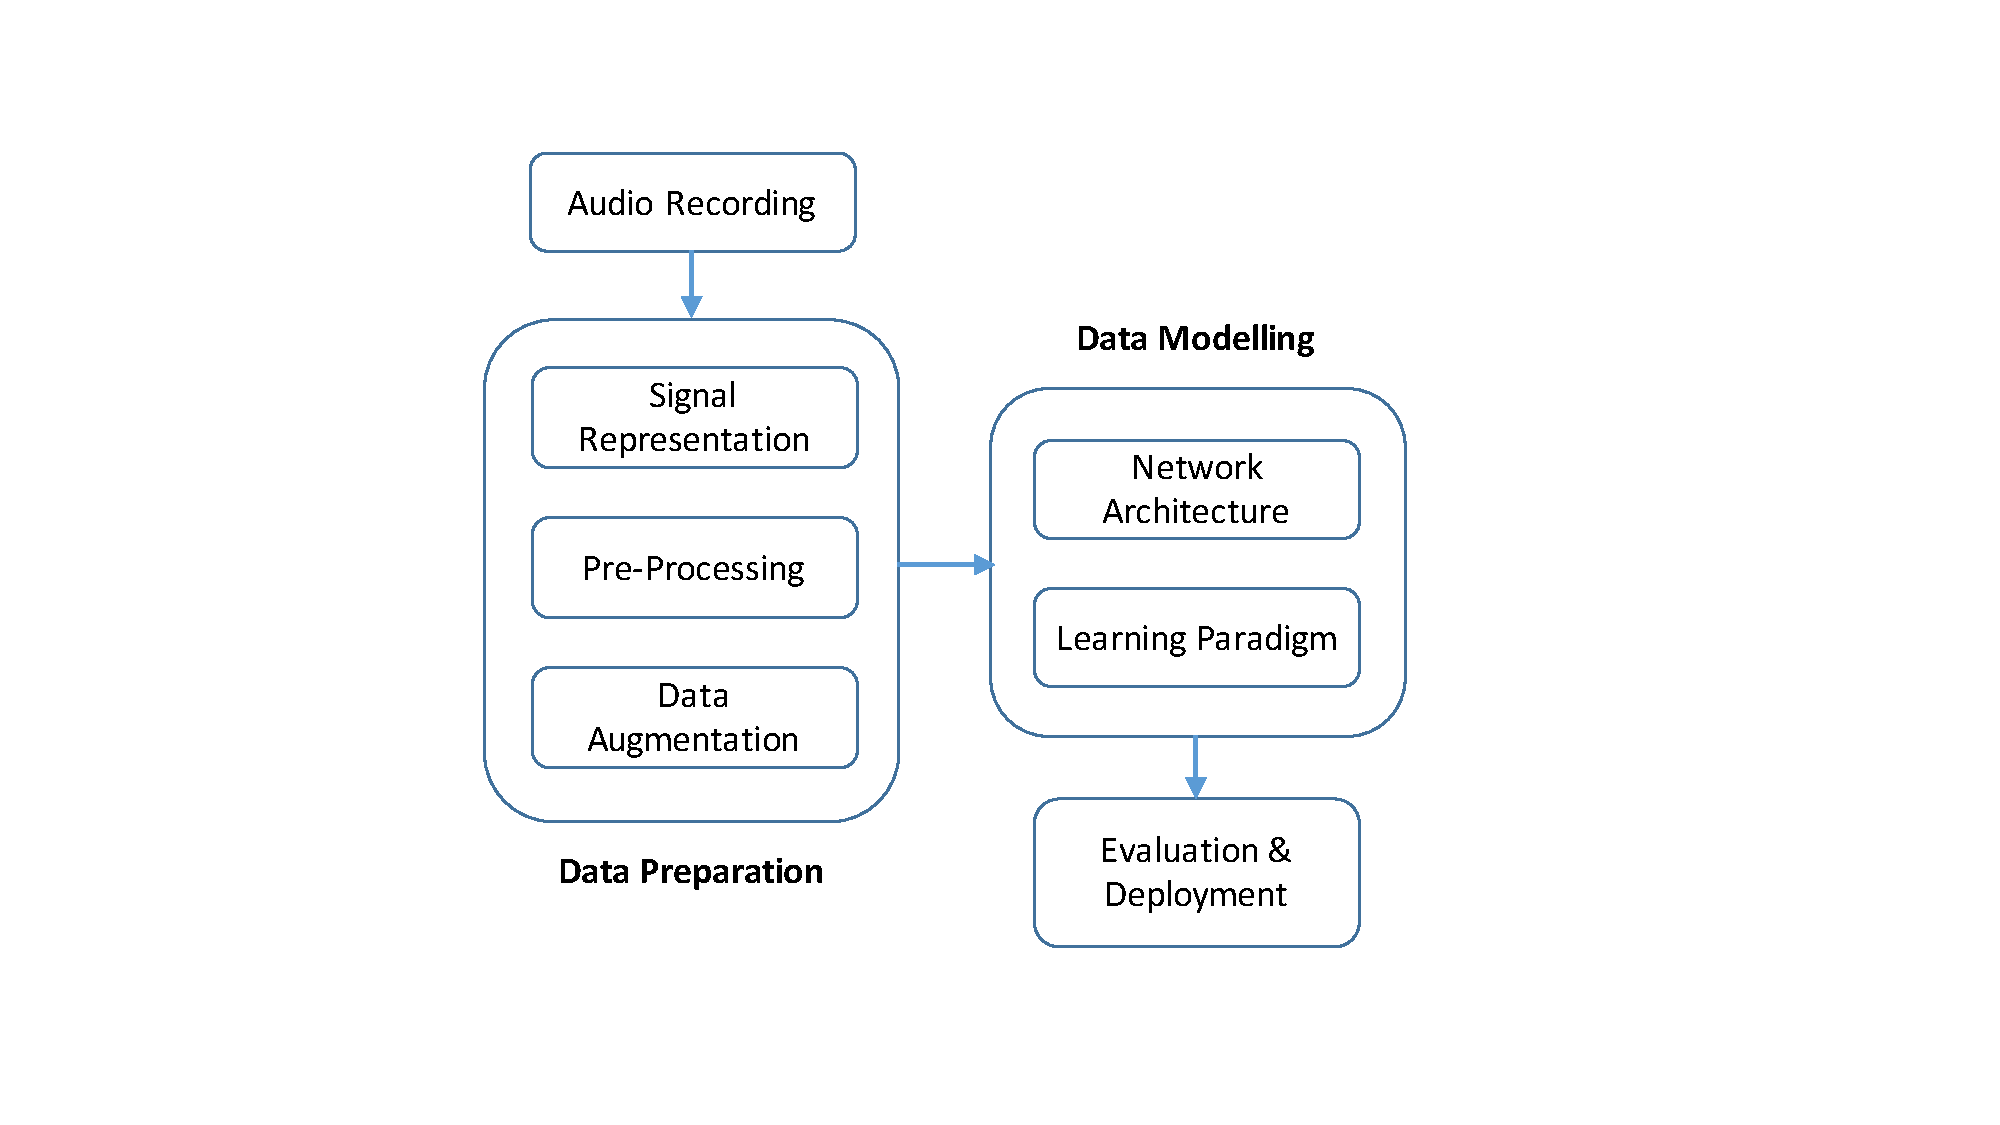
\includegraphics[width=.4\textwidth]{figures/flowchart.pdf}
    \caption{Flowchart summarizes the article structure and lists the typical processing flow of an ASC algorithm.}
\label{fig:flowchart}
\end{figure}


% -------------------------------------
% -------------------------------------
\section{Signal Representations}
\label{sec:feature_representations}
% -------------------------------------
% -------------------------------------
%Designing an ASC algorithm first requires a suitable \textit{feature representation} of the recorded audio signal, which can be further processed by the selected classification algorithm.
%To the best of our knowledge, m
Datasets for the tasks of ASC or AED commonly contain digitized audio recordings. The resulting acoustic signals are commonly represented as waveforms that denote the amplitude of the recorded signal over discrete time samples. In most cases, ASC or AED systems perform the tasks of interest on derived signal representations, which will be introduced in the following section.
%of the above mentioned digitized corpora. We denote this representation, as \textit{feature representation} and is the one that is further processed or analyzed by the corresponding ASC or AED system. 


% -------------------------------------
% -------------------------------------
\subsection{Monaural vs. Multi-Channel Signals}
% -------------------------------------
% -------------------------------------

ASC algorithms commonly process monaural audio signals.
Sound sources in acoustic scenes are spatially distributed by nature.
If multi-channel audio recordings are available, the inherent spatial information can be exploited to better localize sound sources.
The joint localization and detection of sound events has been first addressed in task 3 of the DCASE 2019 challenge.\footnote{\url{http://dcase.community/challenge2019/task-sound-event-localization-and-detection}}

In addition to the left/right channels, a mid/side channel representation can be used as additional signal representation \citep{Han:2017:BinauralASC:DCASE, Mars:2019:BinauralASC:DCASE}.
As an example for using a larger number of audio channels, Green and Murphey \citep{Green:2017:SpatialFeaturesASC:DCASE} classify acoustic scene recordings of 4th-order Ambisonics by combining spatial features describing the direction of sound arrival with band-wise spectral diffuseness measures.
Similarly, Zirli{\'n}ski and Lee combine spatial features from binaural recordings with spectro-temporal features to characterize the foreground/background sound distribution in acoustic scenes \citep{Zielinski:2018:BinauralASC:FEDCSIS}.

 

%\textbf{- ASC for multichannel recordings - bag of acoustic spatial words\citep{Imoto:2017:ASC:EUSIPCO}} 

% take typical locations of sounds in households into account

% -------------------------------------
% -------------------------------------
\subsection{Fixed Signal Transformations}
% -------------------------------------
% -------------------------------------

Most neural network architectures applied for ASC require multi-dimensional input data (compare \secref{sec:network_architectures}). 
The most commonly used time-frequency transformations are the short-time Fourier transform (STFT), 
% TODO Add refs
the mel spectrogram, and the wavelet spectrogram.
The mel spectrogram is based on a non-linear frequency scale motivated by human auditory perception and 
provides a more compact spectral representation of sounds compared to the STFT. 
ASC algorithms process only the magnitude of the Fourier transform while the phase is discarded.

% and transform monaural audio signals into two-dimensional feature representations.
Wavelets can be computed in a one-step \citep{Qian:2017:WaveletASC:DCASE, Ren:2017:DeepSequentialASC:DCASE} or cascaded fashion \citep{Li:2019:MultilevelAttention:ICMEW} to decompose time-domain signals into a set of basis function coefficients.
% Several specialized methods are used as alternatives.
The deep scattering spectrum \citep{Li:2019:MultilevelAttention:ICMEW} decomposes a signal using a sequential cascade of wavelet decompositions and modulation operations.
The scalogram \citep{Chen:2018:Scalogram:INTERSPEECH, Chen:2019:ASC:DCASE} uses multiple parallel wavelet filters with  logarithmically spaced support and bandwidth to provide invariance to both time-warping and local signal translations.
% TODO Piczak shows that using higher number of mel bands usually improves ASC results \citep{Piczak:2017:ASC:DCASE}.
Time-averaged statistics based on computer vision algorithms like Local Binary Patterns (LPB) or Histogram of Oriented Gradients (HOG) can be used to summarize such two-dimensional signal transformations \citep{Ye:2018:ASC:AS}.

In addition to basic time-frequency transformations,
%such low-level signal representations, 
\textit{perceptually-motivated signal representations} are used as input to deep neural networks.
Such representations for instance characterize the distribution (\eg Mel-Frequency Cepstral Coefficients (MFCC) \citep{Li:2018:ASC:ICALIP}, sub-band power distribution \citep{Bisot:2015:ASC:EUSIPCO}, and Gammatone Frequency Cepstral Coefficients \citep{Sharma:2019:SoundClassification:ARXIV}) and modulation of the spectral energy (\eg amplitude modulation bank features \citep{Moritz:2016:TDNN:DCASE} and temporal energy variation \citep{Park:2017:DoubleImageASC:DCASE}). 
Feature learning techniques based on hand-crafted audio features and traditional classification algorithms such as Support Vector Machines (SVM) have been shown to underperform deep learning based ASC algorithms \citep{Fonseca:2017:ASC:DACSE, Maka:2018:FeatureSpaceASC:DCASE}.
% TODO move sentence somewhere else, make point that pre-deep learning classifiers achieve lower classificatio nscores 
% Maka evaluates a large of 223 hand-crafted audio features combined with traditional feature selection and classification algorithms for ASC \citep{Maka:2018:FeatureSpaceASC:DCASE}.
% TODO list examples for classifiers

High-dimensional feature representations are often redundant and can lead to model overfitting. Therefore, before being processed by the neural network, the feature space dimensionality can be further reduced:
One approach is to \textit{aggregate subbands} of spectrograms using local binary pattern (LBP) histograms \citep{Abidin:2017:LBP:ICASSP} or Subband Power Distribution (SBD) features \citep{Bisot:2015:ASC:EUSIPCO}. A second approach is to map features
% TODO what type of features exactly?
 to a randomized low-dimensional feature space as proposed by Jimenez \etal \citep{Jimenez:2017:ShiftInvariantASC:DCASE}.

% TBD (goh) maybe mention embeddings heere as compact features?

% TBD (goh) general note: not sure if this the focus but it would be totally interesting to know what performs "best" right now -> the top5 commonly use mel spec? something like that. Otherwise it reads like some bullet points that you can do anything but have to read and compare all papers to know what is a good starting point . Maybe something like  (just example, don't know what's sota): Raw waveform based approaches have underperformed the commonly used mel spec based representation. However, they bear additional potential since no information such as phase are discarded in the later training process. 

% http://dcase.community/documents/challenge2019/technical_reports/DCASE2019_Zhang_34.pdf

% -------------------------------------
% -------------------------------------
\subsection{Learnable Signal Transformations}
% -------------------------------------
% -------------------------------------


Three different approaches have been used to the best of our knowledge in ASC systems to avoid fixed pre-defined signal transformations.
The first approach is to apply \textit{end-to-end learning} where neural networks directly process raw audio samples. Examples of such network architectures are AclNet and AclSincNet \citep{Huang:2019:ASCEnsemble:DCASE} as well as SoundNet \citep{Singh:2019:MultiViewFeatures:DCASE}. As a potential advantage against spectrogram-based methods, the signal phase is not discarded.
% TODO add citation to original paper ?

The second approach is to interpret the \textit{signal transformation step as learnable function}, commonly denoted as ``front-end'', which can be jointly trained with the classification back-end \citep{Chen:2019:ASCFilters:ICASSP}.
The third approach is to use \textit{unsupervised learning} to derive semantically meaningful signal representations. Amiriparian \etal combine representations learnt using a deep convolutional generative adversarial network (DCGAN) and using a recurrent sequence to sequence autoencoder (S2SAE) \citep{Amiriparian:2018:GANASC:EUSIPCO}. Similarly, environmental audio recordings can be decomposed into suitable basis functions using well-established matrix factorization techniques such Non-Negative Matrix Factorization (NMF) \citep{Bisot:2017:ASC:TASLP} and Shift-Invariant Probabilistic Latent Component Analysis (SIPLCA) \citep{Benetos:2012:ASC:DAFX}.
% TODO add refs



% -------------------------------------
% -------------------------------------
\section{Pre-Processing}
\label{sec:feature_pre_processing}
% -------------------------------------
% -------------------------------------

% TODO decide what to do with that
% Time-frequency feature representations are often cut into overlapping patches of equal duration to enable batch learning. The ASC annotations are simply propagated to the patch-level targets.
%While this procedure allows for more efficient training of the neural network, longer-lasting sound events might not be fully captured within one feature patch.

Feature standardization is commonly used to speed up the convergence of gradient descent based algorithms \citep{Mars:2019:BinauralASC:DCASE}. This process changes the feature distribution to have zero mean and unit variance. 
In order to compensate for the large dynamic range in environmental sound recordings, logarithmic  scaling can be applied to spectrogram based features.
Other low-level audio signal pre-processing methods include dereverberation and low-pass filtering \citep{Seo:2019:ASC:DCASE}.

Both ASC and AED face the challenge that foreground sound events in acoustic scenes are often overshadowed by background noises.
Lostanlen et al. use Per-Channel Energy Normalization (PCEN) \citep{Wang:2017:PCEN:ICASSP} to reduce stationary noise and to enhance transient sound events in environmental audio recordings \citep{Lostanlen:2018:PCEN:SPL}.
This algorithm performs an adaptive, band-wise normalization and decorrelates the frequency bands.
Wu \etal enhance edge-like structures in mel spectrograms using two edge detection methods from image processing based on Difference of Gaussians (DoG) and Sobel filtering \citep{Wu:2019:SoundTexture:ICASSP}. 
The background drift of the mel spectrogram is removed using median filtering.
Similarly, Han \etal use \textit{background subtraction} and apply median filtering over time \citep{Han:2017:BinauralASC:DCASE} to remove irrelevant noise components from the acoustic scene background and the recording device.

Several filtering approaches are used as pre-processing for ASC algorithms.
For example, Nguyen \etal apply a Nearest Neighbor Filter based on the Repeating Pattern Extraction Technique (REPET) algorithm \citep{Rafii:2012:REPET:ISMIR} and replace the most similar spectrogram frames by their median prior to the classification \citep{Nguyen:2018:ASCEnsemble:DCASE}.
This allows to emphasize \textit{repetitive sound} events in acoustic scenes such as from sirens or horns.
As another commonly used filtering approach, 
Harmonic-Percussive Source Separation (HPSS) decomposes the spectrogram into \textit{horizontal and vertical components} and provides additional feature representations for ASC \citep{Han:2017:BinauralASC:DCASE, Mariotti:2018:DeepVisionASC:DCASE, Seo:2019:ASC:DCASE}.

% TBD (goh) also give general recommendation here (what are the best systems using)
% -------------------------------------
% -------------------------------------
\section{Data Augmentation Techniques}
\label{sec:data_augmentation}
% -------------------------------------
% -------------------------------------

Training deep learning models usually requires large amounts of training data to fully capture the natural variability in the data to be modeled.
The size of machine listening datasets increased over the last years but lag behind computer vision datasets such as the ImageNet dataset with over 14 million images and over 21 thousand object classes \citep{Russakovsky:2015:ImageNet:IJCV}.
The only exception to this day is the AudioSet dataset \citep{Gemmeke:2017:Audioset:ICASSP} with currently over 2.1 million audio excerpts and 527 sound event classes.
% TODO any examples / reference for this statement?
This section summarizes techniques for 
\textit{data augmentation} to address this 
lack of data.

% -------------------------------------
% -------------------------------------
%\subsection{Data Modification}
% -------------------------------------
% -------------------------------------

The first group of data augmentation algorithms generates new training data instances from existing ones by applying various signal transformations.
Basic audio signal transformation include \textit{time stretching}, \textit{pitch shifting}, \textit{dynamic range compression}, as well as \textit{adding random noise} \citep{Abesser:2017:ASC:DCASE, Salamon:2017:ASC:SPL, Xu:2018:ASCMobileNet:ISM}. 
Koutini et al. apply \textit{spectral rolling} by randomly shifting spectrogram excerpts over time \citep{Koutini:2019:ReceptiveField:DCASE}.
% TODO ?!? However, it depends on the type of sound, whether it is invariant to pitch shifting.
% TODO any reference for that?

Several data augmentation methods allow to simulate overlap between multiple sound events and the resulting occlusion effects in the spectrogram.
\textit{Mixup} data augmentation allows to create new training instances by mixing pairs of features and their corresponding targets based on a given mixing ratio \citep{Zhang:2018:Mixup:ICLR}. 
Another approach adapted from the computer vision field is \textit{SpecAugment}, where features are temporally warped and blocks of the features are randomly masked \citep{Park:2019:SpecAugment:INTERSPEECH}.
Similarly, \textit{random erasing} involves replacing random boxes in feature representations by random numbers \citep{Zhong:2017:RandomErasing:ARXIV}. 
In the related research task of bird audio detection, Lasseck combines several data augmentation techniques in the time domain (\eg mosaicing random segments, time stretching, time interval dropout) and time-frequency domain (\eg piece-wise time/frequency stretching and shifting) \citep{Lassseck:2018:Bird:DCASE}.




% -------------------------------------
% -------------------------------------
%\subsection{Data Synthesis}
% -------------------------------------
% -------------------------------------

A second group of data augmentation synthesizes novel data instances from scratch. 
The most common synthesis approaches are based on Generative Adversarial Networks (GAN) \citep{Goodfellow:2014:GAN:NIPS}, where class-conditioned synthesis models are trained using an adversarial training strategy by imitating existing data samples.
While data synthesis is usually performed in the audio signal domain \citep{Mun:2017:ASC:ICASSP, Chen:2019:ASC:DCASE}, Mun \etal instead synthesize intermediate embedding vectors \citep{Mun:2017:GANASC:DCASE}.
Kong \etal generate acoustic scenes using the SampleRNN model archictecture \citep{Kong:2019:SceneGeneration:ICASSP}.


% -------------------------------------
% -------------------------------------
\section{Network Architectures}
\label{sec:network_architectures}
% -------------------------------------
% -------------------------------------

ASC algorithms mostly use CNN-based network architectures since they usually provide a summarizing classification of longer acoustic scene excerpts.
In contrast, AED algorithms commonly use convolutional recurrent neural networks (CRNN) as they focus on a precise detection of sound events \citep{Xia:2019:EventDetection:CSSR}.
This architecture combines convolutional neural networks (CNN) as front-end for representation learning and a recurrent layer for temporal modeling. 
Hence, the main focus is on CNN-based ASC methods in \secref{sec:cnn}. Other methods using feedforward neural networks (FNN) and CRNN are briefly discussed in \secref{sec:fnn} and \secref{sec:crnn}, respectively.
Network architectures and the corresponding hyper-parameters are  usually optimized manually.
As an exception, Roletscheck \etal automate this process and compare various architectures, which are automatically generated using a genetic algorithm \citep{Roletscheck:2019:EvolutionaryASC:DCASE}.



% -------------------------------------
% -------------------------------------
\subsection{Convolutional Neural Networks}
\label{sec:cnn}
% -------------------------------------
% -------------------------------------

Traditional CNN architectures use multiple blocks of successive convolution and pooling operations for feature learning and  down-sampling along the time and feature dimensions, respectively.
% TODO quote for that? maybe Deep Learning book?
As an alternative, Ren \etal use \textit{attrous CNNs} which are based on dilated convolutional kernels \citep{Ren:2019:AttrousCNNAttention:ICASSP}. 
Such kernels allow to achieve a comparable \textit{receptive field} size without intermediate pooling operation.
Koutine \etal show that ASC systems can be improved if the receptive field is regularized by restricting its size \citep{Koutini:2019:ASC:DCASE}. 
% TODO any more details here?

In most CNN-based architectures, only the activations of the last convolutional layer are connected to the final classification layers.
As an alternative, Yang \etal follow a \textit{multi-scale feature} approach and further process the activations from all intermediate feature maps \citep{Yang:2018:MultiScaleFeatures:DCASE}.
Additionally, the authors use the Xception network architecture, where the convolution operation is split into a depthwise (spatial) convolution and a pointwise (channel) convolution to reduce the number of trainable parameters.
A related approach is to factorize two-dimensional convolutions into two  one-dimensional kernels to seperately model transient and long-term characteristics of sounds \citep{Cho:DCASE:LargeMarginCNN:DCASE, Sharma:2019:SoundClassification:ARXIV}.
The influence of different symmetric and asymmetric kernel shapes are systematically evaluated by Wang \etal  \citep{Wang:2017:ASC:ISCE}.

Several extensions to the common CNN architeture were proposed to improve the feature learning.
Basbug and Sert adapted the \textit{spatial pyramid pooling} strategy from computer vision, where feature maps are pooled and combined on different spatial resolutions \citep{Basbug:2019:SpatialPyramidPoolingASC:ICSC}.
In order to learn frequency-aware filters in the convolutional layers, Koutini \etal propose to encode the frequency position of each input feature bin within an additional channel dimension (\textit{frequency-aware CNNs}) \citep{Koutini:2019:ReceptiveField:DCASE}.
Similarly, Marchi \etal add the first and second order time derivative of spectrogram-based features as \textit{additional input channels} in order to facilitate detecting transient short-term events which have a rapid increase in magnitude \citep{Marchi:2016:MKSL:DCASE}. 
% TODO: check which spectrogram he used




% -------------------------------------
% -------------------------------------
\subsection{Feedforward Neural Networks}
\label{sec:fnn}
% -------------------------------------
% -------------------------------------

\textit{Feedforward neural networks} (FNN) are used in several ASC algorithms. Bisot \etal use an FNN architecture to concatenate features from an NMF decomposition and a Constant-Q transform of the audio signal \citep{Bisot:2017:NFASC:DCASE}. Takahashi \etal combine an FNN with multiple Gaussian Mixture Model (GMM) classifiers to model the individual acoustic scenes \citep{Takahashi:2017:ASC:APSIPA}.

% -------------------------------------
% -------------------------------------
\subsection{Convolutional Recurrent Neural Networks}
\label{sec:crnn}
% -------------------------------------
% -------------------------------------
The third category of ASC algorithms are based on convolutional recurrent neural networks (CRNN).
Li \etal combine in two separate input branches CNN-based front-ends for feature learning with bidirectional gated recurrent units (BiGRU) for temporal feature modeling  \citep{Li:2019:MultilevelAttention:ICMEW}.
In contrast to a sequential ordering of convolutional and recurrent layers, parallel processing pipelines using long short-term memory (LSTM) layers were used in \citep{Mun:2017:ASC:ICASSP} and \citep{Bae:2016:LSTMCNN:DCASE}.
%Bidirectional recurrent network architectures are often used for ASC \citep{Li:2018:ASC:ICALIP} as the task does not require low-latency / causal classification decisions.
Two recurrent network types used in ASC systems require fewer parameter and less training data compared to LSTM layers---gated recurrent neural networks (GRNN)  \citep{Zoehrer:2016:GRN_ASC:DCASE, Qian:2017:WaveletASC:DCASE, Ren:2017:DeepSequentialASC:DCASE} and time-delay neural networks (TDNN) \citep{Moritz:2016:TDNN:DCASE, Jati:2020:ASC:ICASSP}.


% -------------------------------------
% -------------------------------------
\section{Learning Paradigms}
\label{sec:learning_paradigms}
% -------------------------------------
% -------------------------------------
Building up on the basic neural network architectures introduced in \secref{sec:network_architectures}, approaches to further improve ASC systems are summarized in this section.
After discussing methods for closed/open set classification in \secref{sec:open_closed_set}, extensions to neural networks such as multiple input networks (\secref{sec:multiple_input}) and attention mechanisms (\secref{sec:attention}) are presented.
Finally, both multitask learning (\secref{sec:multitask_learning}) and transfer learning (\secref{sec:transfer_learning}) will be discussed as two promising training strategies to improve ASC systems.

% -------------------------------------
% -------------------------------------
\subsection{Closed/Open Set Classification}
\label{sec:open_closed_set}
% -------------------------------------
% -------------------------------------

Most ASC algorithms assume a \textit{closed-set classification} scenario with a fixed predefined set of acoustic scenes to classify.
In real-world applications however, the underlying data distributions of acoustic scenes is often unknown and can furthermore change over time with new classes becoming relevant.
This motivates the use of \textit{open-set classification} approaches, where an  algorithm can also classify a given audio recording as ``unknown'' class.
This scenario was first addressed as part of the DCASE 2019 challenge in the task 1C ``Open set Acoustic Scene Classification'' \citep{Mesaros:2019:ClosedOpenSet:DCASE}.

Saki \etal propose the \textit{Multi-Class Open-set Evolving Recognition} (MCOSR) algorithm to tackle open-set ASC \citep{Saki:2019:OpenSetASC:DCASE}.
Unknown samples are first rejected by a recognition model before the algorithm tries to identify underlying (hidden) classes in these samples in an unsupervised manner. 
Finally, the recognition model can be updated using the novel classes.
Wilkinghoff and Kurth combine a closed-set classification algorithm and an outlier detection algorithm based on deep convolutional autoencoders (DCAE) to recognize unknown samples in an open-set ASC scenario \citep{Wilkinghoff:2019:OpenSetASC:DCASE}.
Lehner \etal evaluated the model's classification confidence to identify unknown samples \citep{Lehner:2019:ASCReject:DCASE}. Therefore, a threshold is applied on the highest logit value at the input of the final neural network layer.
% TODO check other contributions for this task...

% -------------------------------------
% -------------------------------------
\subsection{Multiple Input Networks}
\label{sec:multiple_input}
% -------------------------------------
% -------------------------------------

As discussed before, most ASC algorithms use a convolutional front-end to learn characteristic patterns in multi-dimensional feature representations. As a general difference to image processing, the time and frequency axes in spectrogram-based feature representations do not carry the same semantic meaning. 
In order to train networks to detect spectral patterns, which are characteristic for certain frequency regions, several authors split a spectrogram into two \citep{Mcdonnell:2019:AcousticScenes:DCASE} or multiple \citep{Phaye:2019:Subspectralnet:ICASSP} sub-bands and use networks with multiple input branches.
Using the same idea of distributed feature learning, other ASC systems individually process the left/right or mid/side channels \citep{Mars:2019:BinauralASC:DCASE} or filtered signal variants, which are obtained using harmonic/percussive separation (HPSS) \citep{Mariotti:2018:DeepVisionASC:DCASE} or nearest neighbor filtering (NNF) \citep{Nguyen:2018:ASCEnsemble:DCASE}.
Instead of feeding multiple signal representations to the network as individual input branches, 
Dang \etal propose to concatenate both MFCC and log mel spectrogram features along the frequency axis as input features \citep{Dang:2018:ASCMulti:ICCE}.

%check goh comments 8.2. 19:38



% -------------------------------------
% -------------------------------------
\subsection{Attention}
\label{sec:attention}
% -------------------------------------
% -------------------------------------
The temporal segments of an environmental audio recording contribute differently to the classification of its acoustic scene.
Neural \textit{attention mechanisms} allow neural networks to focus on a specific subset of its input features.
Attention mechanisms can be incorporated at different positions within neural network based ASC algorithms.
Li \etal incorporate Gated Linear Units (GLU) in several steps of the feature learning part of the network (``multi-level attention'') \citep{Li:2019:MultilevelAttention:ICMEW}.
GLUs implement pairs of mutually gating convolutional layers to  control the information flow in the network.
Attention mechanisms can also be applied in the pooling of feature maps \citep{Ren:2018:AttentionASC:DCASE}.
Wang \etal use self-determination CNNs (SD-CNNs) to identify frames with higher uncertainty due to overlapping sound events. 
A neural network can learn to focus on local patches within the receptive field if a \textit{network-in-network} architecture is used 
\citep{Wang:2018:SelfDeterminationASC:APSIPA}.
Here, individual convolutional layers are extended by micro neural networks, which allows for more powerful approximations by additional non-linearities.

% -------------------------------------
% -------------------------------------
\subsection{Multitask-Learning}
\label{sec:multitask_learning}
% -------------------------------------
% -------------------------------------

\textit{Multitask learning} involves learning to solve multiple related classification tasks jointly with one network \citep{Ruder:2017:MultitaskLearning:ARXIV}.
By learning shared feature representations, the performance on the individual tasks can be improved and a better generalization can be achieved.

A natural approach is to train one model to perform ASC and AED in a joint manner \citep{Bear:2019:JointASCAED:INTERSPEECH} as acoustic events are the building blocks of acoustic scenes.
Sound events and acoustic scenes naturally follow a hierachical relationship.
While most publications perform a ``flat'' classification, Xu \etal exploit a hierarchical acoustic scene taxonomy and group acoustic scenes to the three high-level scene classes ``vehicle'', ``indoor'', and ``outdoor'' \citep{Xu:2016:HierarchicalASC:DCASE}. The authors use a hierarchical pre-training approach, where the network learns to predict the high-level scene class as main task and the low-level scene class such as car or tram as auxiliary task.
Using a similar scene grouping approach, Nwe \etal train a CNN with several shared convolutional layers and three three branches of task-specific convolutional layers to predict the most likely acoustic scene within each scene group \citep{Nwe:2017:MultiTaskASC:APSIPA}.

% -------------------------------------
% -------------------------------------
\subsection{Transfer Learning \& Result Fusion}
\label{sec:transfer_learning}
% -------------------------------------
% -------------------------------------

Many ASC algorithms rely on well proven neural network architectures from the computer vision domain such as AlexNet \citep{Boddapati:2017:ASC:PCS, Ren:2018:AttentionASC:DCASE}, VGG16 \citep{Ren:2017:DeepSequentialASC:DCASE}, Xception \citep{Yang:2018:MultiScaleFeatures:DCASE}, DenseNet \citep{Koutini:2019:ReceptiveField:DCASE}, GoogLeNet \citep{Boddapati:2017:ASC:PCS}, 
and Resnet \citep{Mariotti:2018:DeepVisionASC:DCASE, Lehner:2019:ASCReject:DCASE}.
\textit{Transfer learning} allows the finetuning of models, which were pretrained on related audio classification tasks.
For instance, Huang \etal used the AudioSet dataset to pretrain four different neural network architectures and finetune them using a task-specific development set \citep{Huang:2019:ASCEnsemble:DCASE}. Similarly, Singh et al. take a pretrained SoundNet \citep{Aytar:2016:SoundNet:NIPS} network as basis for their experiments \citep{Singh:2018:EnsembleASC:EUSIPCO, Singh:2019:MultiViewFeatures:DCASE}.
Ren \etal use the VGG16 model as seed model, which was pre-trained for object recognition in images \citep{Ren:2017:DeepSequentialASC:DCASE}. 
Kumar \etal pre-train a CNN in a supervised fashion using weak label annotation of the AudioSet dataset. The authors compare three transfer learning strategies to adapt the model to novel AED and ASC target tasks \citep{Kumar:2018:ASC:ICASSP}.

Many ASC algorithms include \textit{result fusion} steps where intermediate results from different time frames or classifiers are merged.
Similar to computer visions, features learnt in different layers of the network capture different levels of abstraction of the audio signal. Therefore, some systems apply \textit{early fusion} and combine intermediate feature representations from different layers of the network as \textit{multiscale features} \citep{Yang:2018:MultiScaleFeatures:DCASE, Singh:2019:MultiViewFeatures:DCASE, Singh:2018:EnsembleASC:EUSIPCO}.
Ensemble learning is a common \textit{late fusion} technique where the prediction results of multiple classifiers are combined \citep{Ren:2017:DeepSequentialASC:DCASE, Fonseca:2017:ASC:DACSE, Nguyen:2018:ASCEnsemble:DCASE, Huang:2019:ASCEnsemble:DCASE, Mars:2019:BinauralASC:DCASE}.
The predicted class scores can be averaged \citep{Zeinali:2018:XVektorEmbeddings:DCASE} or used as features for an additional classifier  \citep{Weiping:2017:SpectrogramFusion:DCASE}.
%
%% -------------------------------------
%% -------------------------------------
%\section{Datasets}
%% -------------------------------------
%% -------------------------------------
%
%- \textbf{goal: list all available ASC datasets ?!} \\
%- multiple datasets, mostly coming from DCASE challenge, number of classes was reduced from 16 to 10 (...), classes partly overlap \\
%- DCASE 2018 dataset - 10 classes (airport, shopping mall, metro station, street pedestrian, public square, street traffic, tram, bus, metro and park) \\
%
%- multi-device dataset \citep{Mesaros:2018:MultiDeviceDataset:DCASE} \\

% -------------------------------------
% -------------------------------------
\section{Open Challenges}
\label{sec:open_challenges}
% -------------------------------------
% -------------------------------------

This section discusses several open challenges which arise from deploying ASC algorithms to real-world application scenarios.

% -------------------------------------
% -------------------------------------
\subsection{Domain Adapation}
\label{sec:domain_adaptation}
% -------------------------------------
% -------------------------------------

The performance of sound event classification algorithms often suffer from \textit{covariate shift}, \iec a distribution mismatch between training and test datasets.
When being deployed to real-world application scenarios, ASC systems often face novel acoustic conditions which are caused by different recording devices or environmental influences.
\textit{Domain adaption} methods aim to increase the robustness of classification algorithms in such scenarios by adapting them to data from a novel target domain  \citep{Gharib:2018:DomainAdaptationASC:DCASE}.
Depending on whether labels exist for the target domain data, supervised and unsupervised methods are distinguished.
Supervised domain adaptation usually involves fine-tuning a model on a new target domain data after it was pre-trained on the annotated source domain data.

% \textbf{what other supervised methods?} \\
% TBD mention "kernel mean matching (KMM) [13, 14] and autoencoder scheme based approaches [15, 16, 17]" from Gharib paper ?

%Unsupervised domain adaptation involves either altering the distribution of the target domain data or 
One unsupervised domain adaptation strategy is to alter the target domain data such that its distribution becomes closer to that of the source domain data.
As an example, Kosmider use ``spectral correction'' to compensate for different frequency responses of the recording equipment.
He estimates a set of frequency-dependent magnitude coefficients from the source domain data and used them for spectrogram equalization of the target domain data \citep{Kosmider:2019:DeviceCalibration:DCASE}. 
Mun and Shon perform an independent domain adaptation of both the source and target domain to an additional domain using factorized hierarchical variational autoencoder \citep{Mun:2019:DomainMismatch:ICASSP}.

As a second unsupervised strategy, Gharib \etal use an adversarial training approach such that the intermediate feature mappings of an ASC model follow a similar distribution for both the source and target domain data \citep{Gharib:2018:DomainAdaptationASC:DCASE}. This approach is further improved using the Wasserstein generative adversarial networks (WGAN) formulation \citep{Drossos:2019:DomainAdaptation:WASPAA}.


% -------------------------------------
% -------------------------------------
\subsection{Ambiguous Allocation between Sound Events and Scenes}
% -------------------------------------
% -------------------------------------

Acoustic scenes often comprise multiple \textit{sound events}, which are not class-specific but instead appear in a similar way in various scene classes \citep{Park:2017:DoubleImageASC:DCASE, Mesaros:2017:HumanASC:WASPAA}. 
As an example, sound recordings which were recorded in different vehicle types such as car, tram, or train often exhibit \textit{prominent speech} from human conversations or automatic voice announcements. At the same time, class-specific sound components like engine noises, road surface sounds, or door opening and closing sounds  appear at a lower level in the background.
Wu and Lee use the gradient-weighted class activation mappings (GradCAM) to show that CNN-based ASC models in general have the capability to ignore high-energy sound events and focus on quieter background sounds instead \citep{Wu:2019:SoundTexture:ICASSP}.


% -------------------------------------
% -------------------------------------
\subsection{Model Interpretability}
% -------------------------------------
% -------------------------------------

Despite their superior performance, deep learning based ASC models are often considered as ``black boxes'' due to their high complexity and large number of parameters.
One main challenge is to develop methods which allow to better interpret the model predictions and internal feature representations.
As discussed in \secref{sec:attention}, attention mechanisms allow neural networks to focus on relevant subsets of the input data.
Wang \etal investigate an attention-based ASC model and demonstrate that only fractions of long-term scene recordings are relevant for its classification \citep{Wang:2018:SelfDeterminationASC:APSIPA}.
Similarly, Ren \etal visualize internal attention matrices obtained for different acoustic scenes \citep{Ren:2019:AttrousCNNAttention:ICASSP}. The results confirm that either stationary and short-term signal components are most relevant for particular acoustic scenes. 

Another common strategy to investigate the class separability in intermediate feature representations are dimension reduction techniques such as t-SNE \citep{Singh:2019:MultiViewFeatures:DCASE}. 
Techniques such as Layerwise Relevance Propagation (LRP) \citep{Bach:2015:LRP:PLOS} allow to interpret neural networks by investingation the pixel-wise contributions of input features to classification decisions.

% -------------------------------------
% -------------------------------------
\subsection{Real-World Deployment}
% -------------------------------------
% -------------------------------------
Many challenges arise when ASC models are deployed in smart city \citep{Bello:2018:SONYC:CACM, Abesser:2019:Stadtlaerm:DCASE} or industrial sound analysis \citep{Grollmisch:2019:ISA:EUSIPCO} scenarios.
The first challenge is the \textit{model complexity}, which is limited if data privacy concerns require the classification to be performed directly on mobile sensor devices.
\textit{Real-time processing requirements} often demand for fast model prediction with low latency.
In a related study, Sigtia \etal contrast the performance of different audio event detection methods with the respective computational costs \citep{Sigtia:2016:PerformanceCost:IEEE_TASLP}. In comparison to traditional methods such as Support Vector Machines (SVM) and Gaussian Mixture Models (GMM), fully-connected neural networks achive the best performance while requiring the lowest number of operations.

This often requires a \textit{model compression} step, where trained classification models are reduced in size and redundant components need to be identified. 
Several attempts were made to make networks more compact by decreasing the number of operations and increasing the memory-efficiency.
For instance, the MobileNetV2 architecture is based on a novel layer module, which mainly uses convolutional operations to avoid large intermediate tensors
\citep{Sandler:2018:MobileNet:CVPR}.
A similar approach is followed by Drossos \etal for AED \citep{Drossos:2020:SED:ARXIV}. The authors replace the common CNN-based frontend by depthwise separable convolutions and the RNN-backend with dilated convolutions to reduce the number of model parameters and required training time.
In the MorphNet approach proposed by Gordon \etal, network layers are shrunk and expanded in an iterative procedure to optimize network architectures in order to match given resource constraints \citep{Gordon:2018:MorphNet:CVPR}. 
Finally, Tan and Lee show in the EfficientNet approach that a uniform scaling of the network dimensions depth, width, and resolution of a convolutional neural network leads to highly effective networks \citep{Tan:2019:EfficientNet:ICML}.

A second challenge arises from the  \textit{audio recording devices} in mobile sensor units. Due to space constraints, microelectro-mechanical systems (MEMS) microphones are often used.
However, scientific datasets used for training ASC models are usually recorded with high quality electret microphones \citep{Mesaros:2018:MultiDeviceDataset:DCASE}.
As discussed in \secref{sec:domain_adaptation}, changed recording conditions affect the input data distribution. Achieving robust classification systems in such a scenario requires the application of domain adaptation strategies.

% - long-term egocentric audio recordings using smart wearbles \citep{Jati:2020:ASC:ICASSP} \\
% TODO check https://arxiv.org/pdf/2001.08163.pdf

% TODO add "IoT-based Urban Noise Identification Using Machine Learning: Performance of SVM, KNN, Bagging, and Random Forest," COINS '19 Proceedings,
% https://dl.acm.org/citation.cfm?doid=3312614.3312631

% - \textbf{add references from stadtlaerm papers on other iot projects} \\

%- issue was adressed with different recording locations in TAU Urban Acoustic Scenes 2019 dataset \\
% \citep{Singh:2019:MultiViewFeatures:DCASE} \\

% -------------------------------------
% -------------------------------------
% \subsubsection{Other Challenges}
% -------------------------------------
% -------------------------------------


%mis
%\begin{itemize}
 %   \item Evaluation. Is F1 score enough? 
 %   Relevant paper:
 %   "A Framework for the Robust Evaluation of Sound Event Detection"

%    \item Computational Cost: Ecological footprint
%    Relevant paper
%    "Energy and Policy Considerations for Deep Learning in NLP"
%    \item Reproducibility:
%    Other communities already started promoting it:
%    https://reproducibility-challenge.github.io/neurips2019/dates/
    
%\end{itemize}



% -------------------------------------
% -------------------------------------
\section{Conclusion}
\label{sec:conclusion}
% -------------------------------------
% -------------------------------------

% TODO (goh) I'm missing some words about sota -> CNNs with mel and data augmentation? how good are they in general? -> then open challenges

In the research field of acoustic scene classification a rapid increase of scientific publications has been observed in the last decade. This progress was mainly stimulated by recent advances in the field of deep learning such as transfer learning, attention mechanisms, and multitask learning as well as the release of public datasets.
The DCASE community plays a major role in this development by organising annual evaluation campaigns on various machine listening tasks.
%State-of-the-art methods combine data augmentation techniques to enrich the available training data and apply CNN models on log magnitu


% http://dcase.community/challenge2019/task-acoustic-scene-classification-results-a

State-of-the-art ASC algorithms have matured and can be applied in context-aware devices such as hearables and wearables.
In such real-world application scenarios, novel challenges need to be faced such as microphone mismatch and domain adaptation, open set classification, as well as model complexity and real-time processing constraints.
The general demand of deep learning based classification algorithms for larger training corpora can be faced with novel techniques from unsupervised and self-supervised learning as it was shown in natural language processing, speech processing, and image processing.


% %%%%%%%%%%%%%%%%%%%%%%%%%%%%%%%%%%%%%%%%%%
% \setcounter{section}{-1} %% Remove this when starting to work on the template.
% \section{How to Use this Template}
% The template details the sections that can be used in a manuscript. Note that the order and names of article sections may differ from the requirements of the journal (e.g., the positioning of the Materials and Methods section). Please check the instructions for authors page of the journal to verify the correct order and names. For any questions, please contact the editorial office of the journal or support@mdpi.com. For LaTeX related questions please contact latex@mdpi.com.
% %The order of the section titles is: Introduction, Materials and Methods, Results, Discussion, Conclusions for these journals: aerospace,algorithms,antibodies,antioxidants,atmosphere,axioms,biomedicines,carbon,crystals,designs,diagnostics,environments,fermentation,fluids,forests,fractalfract,informatics,information,inventions,jfmk,jrfm,lubricants,neonatalscreening,neuroglia,particles,pharmaceutics,polymers,processes,technologies,viruses,vision

% \section{Introduction}
% The introduction should briefly place the study in a broad context and highlight why it is important. It should define the purpose of the work and its significance. The current state of the research field should be reviewed carefully and key publications cited. Please highlight controversial and diverging hypotheses when necessary. Finally, briefly mention the main aim of the work and highlight the principal conclusions. As far as possible, please keep the introduction comprehensible to scientists outside your particular field of research. Citing a journal paper \citep{ref-journal}. And now citing a book reference \citep{ref-book}. Please use the command \citep{ref-journal} for the following MDPI journals, which use author-date citation: Administrative Sciences, Arts, Econometrics, Economies, Genealogy, Humanities, IJFS, JRFM, Languages, Laws, Religions, Risks, Social Sciences.
 
% %%%%%%%%%%%%%%%%%%%%%%%%%%%%%%%%%%%%%%%%%%
% \section{Results}

% This section may be divided by subheadings. It should provide a concise and precise description of the experimental results, their interpretation as well as the experimental conclusions that can be drawn.
% \begin{quote}
% This section may be divided by subheadings. It should provide a concise and precise description of the experimental results, their interpretation as well as the experimental conclusions that can be drawn.
% \end{quote}

% %%%%%%%%%%%%%%%%%%%%%%%%%%%%%%%%%%%%%%%%%%
% \subsection{Subsection}
% \unskip
% \subsubsection{Subsubsection}

% Bulleted lists look like this:
% \begin{itemize}[leftmargin=*,labelsep=5.8mm]
% \item	First bullet
% \item	Second bullet
% \item	Third bullet
% \end{itemize}

% Numbered lists can be added as follows:
% \begin{enumerate}[leftmargin=*,labelsep=4.9mm]
% \item	First item 
% \item	Second item
% \item	Third item
% \end{enumerate}

% The text continues here.

% \subsection{Figures, Tables and Schemes}

% All figures and tables should be cited in the main text as Figure 1, Table 1, etc.

% \begin{figure}[H]
% \centering
% 
\includegraphics[width=2 cm]{Definitions/logo-mdpi}
% \caption{This is a figure, Schemes follow the same formatting. If there are multiple panels, they should be listed as: (\textbf{a}) Description of what is contained in the first panel. (\textbf{b}) Description of what is contained in the second panel. Figures should be placed in the main text near to the first time they are cited. A caption on a single line should be centered.}
% \end{figure}   
 
% Text

% Text

% \begin{table}[H]
% \caption{This is a table caption. Tables should be placed in the main text near to the first time they are cited.}
% \centering
% %% \tablesize{} %% You can specify the fontsize here, e.g., \tablesize{\footnotesize}. If commented out \small will be used.
% \begin{tabular}{ccc}
% \toprule
% \textbf{Title 1}	& \textbf{Title 2}	& \textbf{Title 3}\\
% \midrule
% entry 1		& data			& data\\
% entry 2		& data			& data\\
% \bottomrule
% \end{tabular}
% \end{table}

% Text

% Text

% %\begin{listing}[H]
% %\caption{Title of the listing}
% %\rule{\textwidth}{1pt}
% %\raggedright Text of the listing. In font size footnotesize, small, or normalsize. Preferred format: left aligned and single spaced. Preferred border format: top border line and bottom border line.
% %\rule{\textwidth}{1pt}
% %\end{listing}


% \subsection{Formatting of Mathematical Components}

% This is an example of an equation:

% \begin{equation}
% a + b = c
% \end{equation}
% %% If the documentclass option "submit" is chosen, please insert a blank line before and after any math environment (equation and eqnarray environments). This ensures correct linenumbering. The blank line should be removed when the documentclass option is changed to "accept" because the text following an equation should not be a new paragraph. 

% Please punctuate equations as regular text. Theorem-type environments (including propositions, lemmas, corollaries etc.) can be formatted as follows:
% %% Example of a theorem:
% \begin{Theorem}
% Example text of a theorem.
% \end{Theorem}

% The text continues here. Proofs must be formatted as follows:

% %% Example of a proof:
% \begin{proof}[Proof of Theorem 1]
% Text of the proof. Note that the phrase `of Theorem 1' is optional if it is clear which theorem is being referred to.
% \end{proof}
% The text continues here.

% %%%%%%%%%%%%%%%%%%%%%%%%%%%%%%%%%%%%%%%%%%
% \section{Discussion}

% Authors should discuss the results and how they can be interpreted in perspective of previous studies and of the working hypotheses. The findings and their implications should be discussed in the broadest context possible. Future research directions may also be highlighted.

% %%%%%%%%%%%%%%%%%%%%%%%%%%%%%%%%%%%%%%%%%%
% \section{Materials and Methods}

% Materials and Methods should be described with sufficient details to allow others to replicate and build on published results. Please note that publication of your manuscript implicates that you must make all materials, data, computer code, and protocols associated with the publication available to readers. Please disclose at the submission stage any restrictions on the availability of materials or information. New methods and protocols should be described in detail while well-established methods can be briefly described and appropriately cited.

% Research manuscripts reporting large datasets that are deposited in a publicly available database should specify where the data have been deposited and provide the relevant accession numbers. If the accession numbers have not yet been obtained at the time of submission, please state that they will be provided during review. They must be provided prior to publication.

% Interventionary studies involving animals or humans, and other studies require ethical approval must list the authority that provided approval and the corresponding ethical approval code. 

% %%%%%%%%%%%%%%%%%%%%%%%%%%%%%%%%%%%%%%%%%%
% \section{Conclusions}

% This section is not mandatory, but can be added to the manuscript if the discussion is unusually long or complex.

% %%%%%%%%%%%%%%%%%%%%%%%%%%%%%%%%%%%%%%%%%%
% \section{Patents}
% This section is not mandatory, but may be added if there are patents resulting from the work reported in this manuscript.

% %%%%%%%%%%%%%%%%%%%%%%%%%%%%%%%%%%%%%%%%%%
% \vspace{6pt} 

%%%%%%%%%%%%%%%%%%%%%%%%%%%%%%%%%%%%%%%%%%
%% optional
%\supplementary{The following are available online at \linksupplementary{s1}, Figure S1: title, Table S1: title, Video S1: title.}

% Only for the journal Methods and Protocols:
% If you wish to submit a video article, please do so with any other supplementary material.
% \supplementary{The following are available at \linksupplementary{s1}, Figure S1: title, Table S1: title, Video S1: title. A supporting video article is available at doi: link.}

% %%%%%%%%%%%%%%%%%%%%%%%%%%%%%%%%%%%%%%%%%%
% \authorcontributions{For research articles with several authors, a short paragraph specifying their individual contributions must be provided. The following statements should be used ``conceptualization, X.X. and Y.Y.; methodology, X.X.; software, X.X.; validation, X.X., Y.Y. and Z.Z.; formal analysis, X.X.; investigation, X.X.; resources, X.X.; data curation, X.X.; writing--original draft preparation, X.X.; writing--review and editing, X.X.; visualization, X.X.; supervision, X.X.; project administration, X.X.; funding acquisition, Y.Y.'', please turn to the  \href{http://img.mdpi.org/data/contributor-role-instruction.pdf}{CRediT taxonomy} for the term explanation. Authorship must be limited to those who have contributed substantially to the work reported.}

%%%%%%%%%%%%%%%%%%%%%%%%%%%%%%%%%%%%%%%%%%
\funding{This work has received funding from the European Union's Horizon 2020 research and innovation programme under grant agreement No 786993 and was supported by the German Research Foundation (\mbox{AB 675/2-1}).

}

%%%%%%%%%%%%%%%%%%%%%%%%%%%%%%%%%%%%%%%%%%
\acknowledgments{
%In this section you can acknowledge any support given which is not covered by the author contribution or funding sections. This may include administrative and technical support, or donations in kind (e.g., materials used for experiments).
The author would like to thank Hanna Lukashevich, Stylianos Mimilakis, David S. Johnson,  and Sascha Grollmisch for valuable discussions and proof-reading.
}

%%%%%%%%%%%%%%%%%%%%%%%%%%%%%%%%%%%%%%%%%%
\conflictsofinterest{
The author declares no conflict of interest.
%Declare conflicts of interest or state ``The authors declare no conflict of interest.'' Authors must identify and declare any personal circumstances or interest that may be perceived as inappropriately influencing the representation or interpretation of reported research results. Any role of the funders in the design of the study; in the collection, analyses or interpretation of data; in the writing of the manuscript, or in the decision to publish the results must be declared in this section. If there is no role, please state ``The funders had no role in the design of the study; in the collection, analyses, or interpretation of data; in the writing of the manuscript, or in the decision to publish the results''.
} 

%%%%%%%%%%%%%%%%%%%%%%%%%%%%%%%%%%%%%%%%%%
%% optional
%\abbreviations{The following abbreviations are used in this manuscript:\\

%\noindent 
%\begin{tabular}{@{}ll}
%AED & Acoustic Event Detection \\
%ASC & Acoustic Scene Classification \\
%CNN & Convolutional Neural Network\\
%CRNN & Convolutional Recurrent Neural Network \\
%DCASE & Detection and Classification  of  Acoustic  Scenes  and  Event\\
%IoT & Internet of Things \\
%STFT & Short-Time Fourier Transform \\
%\end{tabular}}

%%%%%%%%%%%%%%%%%%%%%%%%%%%%%%%%%%%%%%%%%%
%% optional
%\appendixtitles{no} %Leave argument "no" if all appendix headings stay EMPTY (then no dot is printed after "Appendix A"). If the appendix sections contain a heading then change the argument to "yes".
%\appendix
%\section{}
%\unskip
%\subsection{}
%The appendix is an optional section that can contain details and data supplemental to the main text. For example, explanations of experimental details that would disrupt the flow of the main text, but nonetheless remain crucial to understanding and reproducing the research shown; figures of replicates for experiments of which representative data is shown in the main text can be added here if brief, or as Supplementary data. Mathematical proofs of results not central to the paper can be added as an appendix.


%%%%%%%%%%%%%%%%%%%%%%%%%%%%%%%%%%%%%%%%%%
% Citations and References in Supplementary files are permitted provided that they also appear in the reference list here. 

%=====================================
% References, variant A: internal bibliography
%=====================================
\reftitle{References}


% The following MDPI journals use author-date citation: Arts, Econometrics, Economies, Genealogy, Humanities, IJFS, JRFM, Laws, Religions, Risks, Social Sciences. For those journals, please follow the formatting guidelines on http://www.mdpi.com/authors/references
% To cite two works by the same author: \citep{ref-journal-1a} (\citeyear{ref-journal-1a}, \citeyear{ref-journal-1b}). This produces: Whittaker (1967, 1975)
% To cite two works by the same author with specific pages: \citep{ref-journal-3a} (\citeyear{ref-journal-3a}, p. 328; \citeyear{ref-journal-3b}, p.475). This produces: Wong (1999, p. 328; 2000, p. 475)

%=====================================
% References, variant B: external bibliography
%=====================================
\externalbibliography{yes}
\bibliography{refs_clean_red_3}

%%%%%%%%%%%%%%%%%%%%%%%%%%%%%%%%%%%%%%%%%%
%% optional
%\sampleavailability{Samples of the compounds ...... are available from the authors.}

%% for journal Sci
%\reviewreports{\\
%Reviewer 1 comments and authors’ response\\
%Reviewer 2 comments and authors’ response\\
%Reviewer 3 comments and authors’ response
%}

%%%%%%%%%%%%%%%%%%%%%%%%%%%%%%%%%%%%%%%%%%
\end{document}

